\documentclass[a4paper]{article}
\usepackage[english]{babel}
\usepackage[top=1.1cm,headsep=0cm,bottom=1.1cm,footskip=0cm,left=1cm,right=1cm]{geometry}
\usepackage{multicolrule} %다단 본문
\usepackage{fontspec}
\setmathtt{exprdgs-italic.ttf}[BoldFont = exprdgs-bolditalic.ttf]
\usepackage[colorlinks=true, allcolors=black]{hyperref}
\usepackage{wrapfig} %문단 내 이미지 삽입
\usepackage[abs]{overpic} %이미지 위 텍스트 삽입
\usepackage{graphicx,color} %색상
\usepackage[normalem]{ulem}%취소선
\usepackage{array} %표
\usepackage{mdframed, tcolorbox} %글상자
\usepackage{amsmath, amsfonts, amssymb, bm} %수식

\DeclareMathOperator{\arccsc}{arccsc}
\DeclareMathOperator{\arcsec}{arcsec}
\DeclareMathOperator{\arccot}{arccot}
\DeclareMathOperator{\csch}{csch}
\DeclareMathOperator{\sech}{sech}
\DeclareMathOperator{\arcsinh}{arcsinh}
\DeclareMathOperator{\arccosh}{arccosh}
\DeclareMathOperator{\arctanh}{arctanh}
\DeclareMathOperator{\arccsch}{arccsch}
\DeclareMathOperator{\arcsech}{arcsech}
\DeclareMathOperator{\arccoth}{arccoth}

\DeclareMathOperator{\snd}{s}
\DeclareMathOperator{\meter}{m}
\DeclareMathOperator{\cm}{cm}
\DeclareMathOperator{\mm}{mm}
\DeclareMathOperator{\mum}{\mu m}

\DeclareMathOperator{\newton}{N}
\DeclareMathOperator{\kn}{kN}
\DeclareMathOperator{\kgf}{kgf}

\DeclareMathOperator{\pa}{Pa}
\DeclareMathOperator{\kpa}{kPa}
\DeclareMathOperator{\mpa}{MPa}
\DeclareMathOperator{\gpa}{GPa}
\DeclareMathOperator{\mmhg}{mmHg}
\DeclareMathOperator{\knpm}{kN/m}

\DeclareMathOperator{\mps}{m/s}
\DeclareMathOperator{\mpss}{m/s^2}

\DeclareMathOperator{\dgr}{\!^\circ}
\DeclareMathOperator{\cel}{\!^\circ C}
\DeclareMathOperator{\fer}{\!^\circ F}
\DeclareMathOperator{\kel}{K}

\DeclareMathOperator{\kg}{kg}
\DeclareMathOperator{\kgpcm}{kg/m^3}
\DeclareMathOperator{\cmpkg}{m^3/kg}

\DeclareMathOperator{\nm}{N\cdot m}

\DeclareMathOperator{\watt}{W}
\DeclareMathOperator{\kw}{kW}
\DeclareMathOperator{\kwh}{kWh}

\DeclareMathOperator{\joule}{J}
\DeclareMathOperator{\kj}{kJ}
\DeclareMathOperator{\jpkg}{J/kg}
\DeclareMathOperator{\kjpkg}{kJ/kg}
\DeclareMathOperator{\kjpkk}{kJ/kg\cdot K}
\DeclareMathOperator{\kjpk}{kJ/K}
\DeclareMathOperator{\kps}{kg/s}

\DeclareMathOperator{\satat}{sat\,@}
\DeclareMathOperator{\supat}{sup\,@}
\DeclareMathOperator{\comat}{com\,@}

\usepackage{polynom} %나눗셈 필산
\usepackage{cancel} %수식 약분선
\usepackage{titlesec} %섹션 이름 변경
\usepackage{kotex} %한글
\usepackage{fancyhdr} %페이지 넘버 편집
\pagestyle{fancy}
\renewcommand{\headrulewidth}{0pt}
\fancyhf{}
\fancyhead[R]{p.\thepage}
\fancyfoot[R]{\color{red}[\LaTeX]}

\setlength\columnsep{2cm}
\SetMCRule{
	width = 0.3mm,
	color-model = rgb,
	color = {0.9,0.9,0.9},
	line-style = dashed
}

\renewcommand{\section}[1] {
	\vspace{\baselineskip}
	\noindent\hspace{-1.0cm}\begin{overpic}{qframe.png}
		\put(8mm,-0.3mm){
			\begin{tcolorbox}[
				boxsep = 0mm,
				top = 0mm,
				bottom = 0mm,
				left = 0mm,
				right = 0mm,
				boxrule = 0mm,
				colback = white,
				colframe = blue,
				width = 2.2cm,
				height = 8mm,
				halign = center,
				valign = center,
				sharp corners = all,
				opacityfill = 0,
				fontupper = \bfseries
				]
				{[ #1 ]}
			\end{tcolorbox}
		}
	\end{overpic}
}

\makeatletter
\renewcommand{\maketitle}{\setlength{\parindent}{0pt}
	\begin{flushleft}
		\LARGE{\textbf{\@title}}\\
		\vspace{0.6cm}
		\LARGE{\qquad\@author}
		\vspace{0.5cm}
	\end{flushleft}
	\hspace{-1cm}\noindent\textcolor{red}{\rule{21cm}{0.5mm}}
}
\makeatother

\newcommand{\asw}[2]{
	\begin{flushright}
		{#1 \quad #2 \quad $\blacktriangleleft$}
	\end{flushright}
}

\newcommand{\solution}{\noindent\textbf{[풀이]}}

\title{열역학(이상훈 교수님)\hspace{5cm} 2023-1 기말고사 풀이}
\author{기계공학부,\qquad 2022****,\qquad 2학년,\qquad ***}
\date{}

\begin{document}

\maketitle

\begin{multicols*}{2}

\setlength{\parindent}{3mm}

\section{Q1-4}
	아래 열역학 용어들을 영어로 쓰시오.\\[10pt]
	-열효율 : thermal efficiency\\
	-C.O.P. : coefficient of performance\\
	-비가역상태 : irreversible\\
	-등엔트로피 과정 : isentropic process

\section{Q5}
	Kelvin-Plank 서술을 정의하시오.\\
	
	닫힌 과정에서 작동하는 열기관이 하나의 열원으로부터 열을 전달받아 정미일을 생산해 내는 것은 불가능하다.
	
\section{Q6}
	카르노의 원리 1번을 서술하시오.\\
	
	두 열원 사이에서 작동하는 모든 실제 열기관들의 열효율은 같은 열원 사이에서 작동하는 카르노 기관의 열효율을 넘을 수 없다.
	
\section{Q7}
	정상상태, 단일류, 개방시스템일 때 단위질량 당으로 표현한 ($a$) 열역학 제 1법칙, ($b$) 2법칙에 대한 식과 ($b$) 질량보존식을 쓰시오.
	\asw{($a$)}{$q + h_i + \frac{V_i^2}{2} + gz_i = h_e + \frac{V_e^2}{2} + gz_e + w$}
	\asw{($b$)}{$s_e = s_i + \sum \frac{q_k}{T_k} + \theta$}
	\asw{($c$)}{$\dot{m}_i = \dot{m}_e$}

\section{Q8}
	$0.6\mpa$의 포화증기 상태의 수증기가 단열 팽창 밸브를 통과해서 $0.3\mpa$이 되었을 때, 밸브를 통과한 후의 수증기의 상태를 정량적으로 결정하시오. (수치에 근거하여)\\
	
	\solution
	\begin{align*}
		&\cancel{q} + h_1 = h_2 + \cancel{w}\\
		&h_1 = h_{g,\satat 600\kpa} = 2756.2\kjpkg = h_2\\
		&h_{g,\satat 300\kpa} = 2724.9\kjpkg < h_2 \quad\Rightarrow\quad \text{과열증기}
	\end{align*}
	\asw{}{과열증기}

\section{Q9}
	카르노 기관의 정의에 대해 서술하고 $T$-$s$선도에 카르노 선도를 나타내시오.\\
	
	두 개의 가역 단열과정과 두 개의 등온과정으로 이루어진 사이클 상에서 작동하는 이상적인 열기관
	\begin{center}
		\includegraphics[width = 60mm]{img/fig7-19.png}
	\end{center}
	
\section{Q10}
	$80\cel$의 열원에서 $25\cel$의 열원으로 열이 방출될 때, 카르노 효율과 카르노 냉동기의 성능 계수를 구하시오.\\
	
	\solution
	\begin{align*}
		&T_H = 80 + 273.15 = 353.15000 \approx 353.15\kel\\
		&T_H = 25 + 273.15 = 298.15000 \approx 298.15\kel\\
		&\eta_{\text{rev}} = \frac{W}{Q_H} = 1 - \frac{Q_L}{Q_H} = 1 - \frac{T_L}{T_H}\\
		&\quad = 1 - \frac{298.15}{353.15} = 0.15574119 \approx 0.156\\
		&\text{COP}_\text{R} = \frac{Q_L}{W} = \frac{1}{\frac{Q_H}{Q_L} - 1} = \frac{1}{\frac{T_H}{T_L} - 1}\\
		&\quad = \frac{1}{\frac{353.15}{298.15} - 1} = 5.42090909 \approx 5.42
	\end{align*}
	\asw{}{$0.156\,;\,5.42$}

\section{Q11}
	초기 압력 $3\mpa$, 초기 온도 $270\cel$인 질량이 $5\kg$인 공기가 $n=1.25$인 폴리트로픽 과정에 의해 압력이 $0.5\mpa$이 된다. 이때 ($a$) 최종 온도, ($b$) 과정에서 공기가 한 일, ($c$) 엔트로피 변화를 구하시오.\\
	
	\solution
	\begin{align*}
		&TP^{\frac{1-n}{n}} = \text{const.}\;\Rightarrow\; T_1P_1^{\frac{1-n}{n}} = T_2P_2^{\frac{1-n}{n}}\\
		&T_2 = T_1\left(\frac{P_1}{P_2}\right)^{\frac{1-n}{n}} = 543.15\left(\frac{3000}{500}\right)^{\frac{1-1.25}{1.25}}\\
		&\quad = 379.56794956 \approx 379.57\kel = 106.42\cel
	\end{align*}
	\asw{($a$)}{$106.42\cel$}
	\begin{align*}
		&W_{12} = m\frac{P_2\mathtt{v}_2 - P_1\mathtt{v}_1}{1-n} = \frac{mR\left(T_2 - T_1\right)}{1-n}\\
		&\quad = \frac{(5)(0.2870)(379.57-543.15)}{1 - 1.25} = 938.9492000\\
		&\quad \approx 938.949\kj
	\end{align*}
	\asw{($b$)}{$938.949\kj$}
	\begin{align*}
		&\Delta S = mR\left(\frac{\kappa}{\kappa - 1}\ln\frac{T_2}{T_1} - \ln\frac{P_2}{P_1}\right)\\
		&\quad = (5)(0.2870)\left(\frac{1.4}{1.4-1}\ln\frac{379.57}{543.15} - \ln\frac{500}{3000}\right)\\
		&\quad = 0.7713795831 \approx 0.771\kjpk
	\end{align*}
	\asw{($c$)}{$0.771\kjpk$}
	
\section{Q12}
	초기 압력 $3\mpa$, 초기 온도 $350\cel$, 초기 속도 $50\mps$인 수증기가 터빈을 통과해 최종압력은 $0.1\mpa$인 습증기가 되었다. 이때의 건도는 $92\%$이며 최종속도는 $180\mps$이다. 질량유량은 $2\kps$이며 손실열은 $15\kw$이다. ($a$) 에너지 보존식과 질량 보존식, ($b$) 축 일, ($c$) 엔탈피의 변화량을 구하시오.\\
	
	\solution
	
	\asw{($a$)}{\begin{tabular}{r}
		$\dot{Q} + \dot{m}_1\left(h_1 + \frac{V_1^2}{2}\right) = \dot{m}_2\left(h_2 + \frac{V_2^2}{2}\right) + \dot{W}$\\[10pt]
		$\dot{m}_1 = \dot{m}_2$
	\end{tabular}}
	\begin{align*}
		&T_{\satat 3\mpa} = 233.85\cel < T_1 = 350\cel\;\Rightarrow\; \text{과열증기}\\
		&h_1 = h_{@3\mpa,350\cel} = 3116.1\kjpkg\\
		&h_{2f} = h_{f,\satat 100\kpa} = 417.51\kjpkg\\
		&h_{2fg} = h_{fg,\satat 100\kpa} = 2257.5\kjpkg\\
		&h_2 = h_{2f} + x_2h_{2fg} = 417.51 + (0.92)(2257.5)\\
		&\quad = 2494.41000 \approx 2494.410\kjpkg\\
		&\dot{m} = \dot{m}_1 = \dot{m}_2\\
		&\dot{Q} + \dot{m}\left(h_1 + \frac{V_1^2}{2}\right) = \dot{m}\left(h_2 + \frac{V_2^2}{2}\right) + \dot{W}\\
		&\dot{W} = \dot{Q} + \dot{m}\left(h_1 - h_2 + \frac{V_1^2 - V_2^2}{2}\right)\\
		&\quad = -15 + (2)\left(3116.1 - 2494.41 + \frac{50^2 - 180^2}{2}\times10^{-3}\right)\\
		&\quad = 1198.48000 \approx 1198.480\kw
	\end{align*}
	\asw{($b$)}{$1198.480\kw$}
	\begin{align*}
		&\Delta h = h_2 - h_1 = 2494.41 - 3116.1\\
		&\quad = -621.69\kjpkg
	\end{align*}
	\asw{($c$)}{$-621.69\kjpkg$}
	
	
\section{Q13}
	정상유동의 $150\kpa$의 열 혼합기 안에서 $70\cel$의 물과 $15\cel$의 물을 혼합해 $45\cel$가 될 때, $70\cel$의 물과 $15\cel$의 물의 질량유량의 비율을 $y$라고 하자. ($y>1$) 이때 ($a$) 질량 보존식과 에너지 보존식을 구하시오. ($b$) $y$에 대한 식을 유도하고 $y$의 값을 구하시오.\\
	
	\solution
	\begin{align*}
		&P = 150\kpa,\quad T_1 = 70\cel,\quad T_2 = 15\cel,\quad \dot{m}_1 = y\dot{m}_2\\
		&\sum_i m = \sum_e m \quad\Rightarrow\quad \dot{m}_1 + \dot{m}_2 = \dot{m}_e\\
		&\cancel{\dot{Q}} + \sum_i \dot{m}j = \sum_e \dot{m}j + \cancel{\dot{W}} \;\Rightarrow\; \dot{m}_1h_1 + \dot{m}_2h_2 = \dot{m}_eh_e
	\end{align*}
	\asw{($a$)}{$\dot{m}_1 + \dot{m}_2 = \dot{m}_e\,;\,\dot{m}_1h_1 + \dot{m}_2h_2 = \dot{m}_eh_e$}
	\begin{align*}
		&T_{\satat 150\kpa} = 111.35\cel > T_1 > T_e > T_2 \;\Rightarrow\;\text{압축액}\\
		&h_1 \approx h_{f,\satat 70\cel} = 293.07\kjpkg\\
		&h_2 \approx h_{f,\satat 15\cel} = 62.982\kjpkg\\
		&h_e \approx h_{f,\satat 45\cel} = 188.44\kjpkg\\
		&y\dot{m}_2h_1 + \dot{m}_2h_2 = (y\dot{m}_2 + \dot{m}_2)h_e\\
		&yh_1 + h_2 = (y+1)h_e\\
		&y = \frac{h_e - h_2}{h_1 - h_e} = \frac{188.44 - 62.982}{293.07 - 188.44} = 1.19906337 \approx 1.199
	\end{align*}
	\asw{($b$)}{$1.199$}
	
\section{Q14}
	아래 그림의 단열된 파이프와 밸브로 연결된 탱크에 대하여 ($a$) 질량보존식과 에너지 보존식을 구하시오. ($b$) $a$에서 구한 식을 이용하여 탱크 안으로 유입된 공기의 온도를 구하는 공식을 유도하시오. (단, 최종 계산 전까지 식을 정리하지 말고 $du=c_\mathtt{v}dT$, $dh=c_pdT$를 사용하지 마시오) ($
	c$) 최종 온도를 구하시오.
	\begin{center}
		\includegraphics{img/q14-0.png}
	\end{center}
	\solution
	\begin{align*}
		&\sum_i m - \cancel{\sum_e m} = (\Delta m)_{\text{CV}} = m_2 - \cancel{m_1}\;\Rightarrow\;m_i = m_2\\
		&\cancel{Q} + \sum_i mj - \cancel{\sum_e mj} - \cancel{W} = (\Delta E)_{\text{CV}} = m_2e_2 - \cancel{m_1e_1}\\
		&\Rightarrow \; m_ih_i = m_2u_2
	\end{align*}
	\asw{($a$)}{$m_i = m_2\,;\,m_ih_i = m_2u_2$}
	\begin{align*}
		&m_1h_1 = m_1u_2 \quad\Rightarrow\quad h_1 = u_2
	\end{align*}
	 \begin{tabular}{|c|c|}
		\hline
		$T\,[\kel]$ & $h\,[\kjpkg]$\\
		\hline
		520.00 & 523.63\\
		523.15 & $h_1$\\
		530.00 & 533.98\\
		\hline
	\end{tabular}\quad$\cdots$\quad(Table A-17)\\
	\begin{align*}
		&h_1 = \cfrac{523.15 - 520}{530 - 520}(533.98 - 523.63) + 523.63\\
		&\quad = 526.89025000 \approx 526.890\kjpkg
	\end{align*}
	\begin{tabular}{|c|l|}
		\hline
		$T\,[\kel]$ & $u\,[\kjpkg]$\\
		\hline
		710.00 & 520.23\\
		$T_2$ & 526.89\;($u_2$)\\
		720.00 & 528.14\\
		\hline
	\end{tabular}\quad$\cdots$\quad(Table A-17)\\
	\begin{align*}
		&T_2 = \cfrac{526.89 - 520.23}{528.14 - 520.23}(720 - 710) + 710\\
		&\quad = 718.4197219 \approx 718.420\kel
	\end{align*}
	
	
\section{Q15}
	공기가 최초온도 300K와 최종압력 100kPa에서 최종온도 400K 최종압력 700kPa으로 변할 때 ($a$) 공기표에서 얻은 상태량의 값으로 엔트로피 변화를 구하시오. ($b$) 평균 비열을 이용해 엔트로피 변화를 구하시오.\\
	
	\solution
	\begin{align*}
		&ds = \frac{c_p}{T}dT - \frac{R}{P}dP\\
		&s_2 - s_1 = \int^2_1 \frac{c_p}{T}dT - \int^2_1 \frac{R}{P}dP\\
		&\quad  = s^\text{o}(T_2) - s^\text{o}(T_1) - R\ln\frac{P_2}{P_1}\\
		&\quad = 1.99194 - 1.70203 - (0.2870)\ln\frac{700}{100}\\
		&\quad = -0.2685662128 \approx -0.269\kjpkk
	\end{align*}
	\asw{($a$)}{$-0.269\kjpkk$}
	\begin{align*}
		&c_{p,@300\kel} = 1.005\kjpkk\\
		&c_{p,@400\kel} = 1.013\kjpkk\\
		&c_{p,\text{avg}} = \frac{c_{p,@300\kel} + c_{p,@400\kel}}{2} = \frac{1.005 + 1.013}{2}\\
		&\qquad = 1.009000 \approx 1.009\kjpkk\\
		&s_2 - s_1 = c_{p,\text{avg}}\ln\frac{T_2}{T_1} - R\ln\frac{P_2}{P_1}\\
		&\quad = (1.009)\ln\frac{400}{300} - (0.2870)\ln\frac{700}{100}\\
		&\quad = -0.2682050017 \approx -0.268\kjpkk
	\end{align*}
	\asw{($b$)}{$-0.268\kjpkk$}

\end{multicols*}
\end{document}